
Transforming circuit to the frequency (s) domain:\\

\begin{figure}[H]
\begin{center}
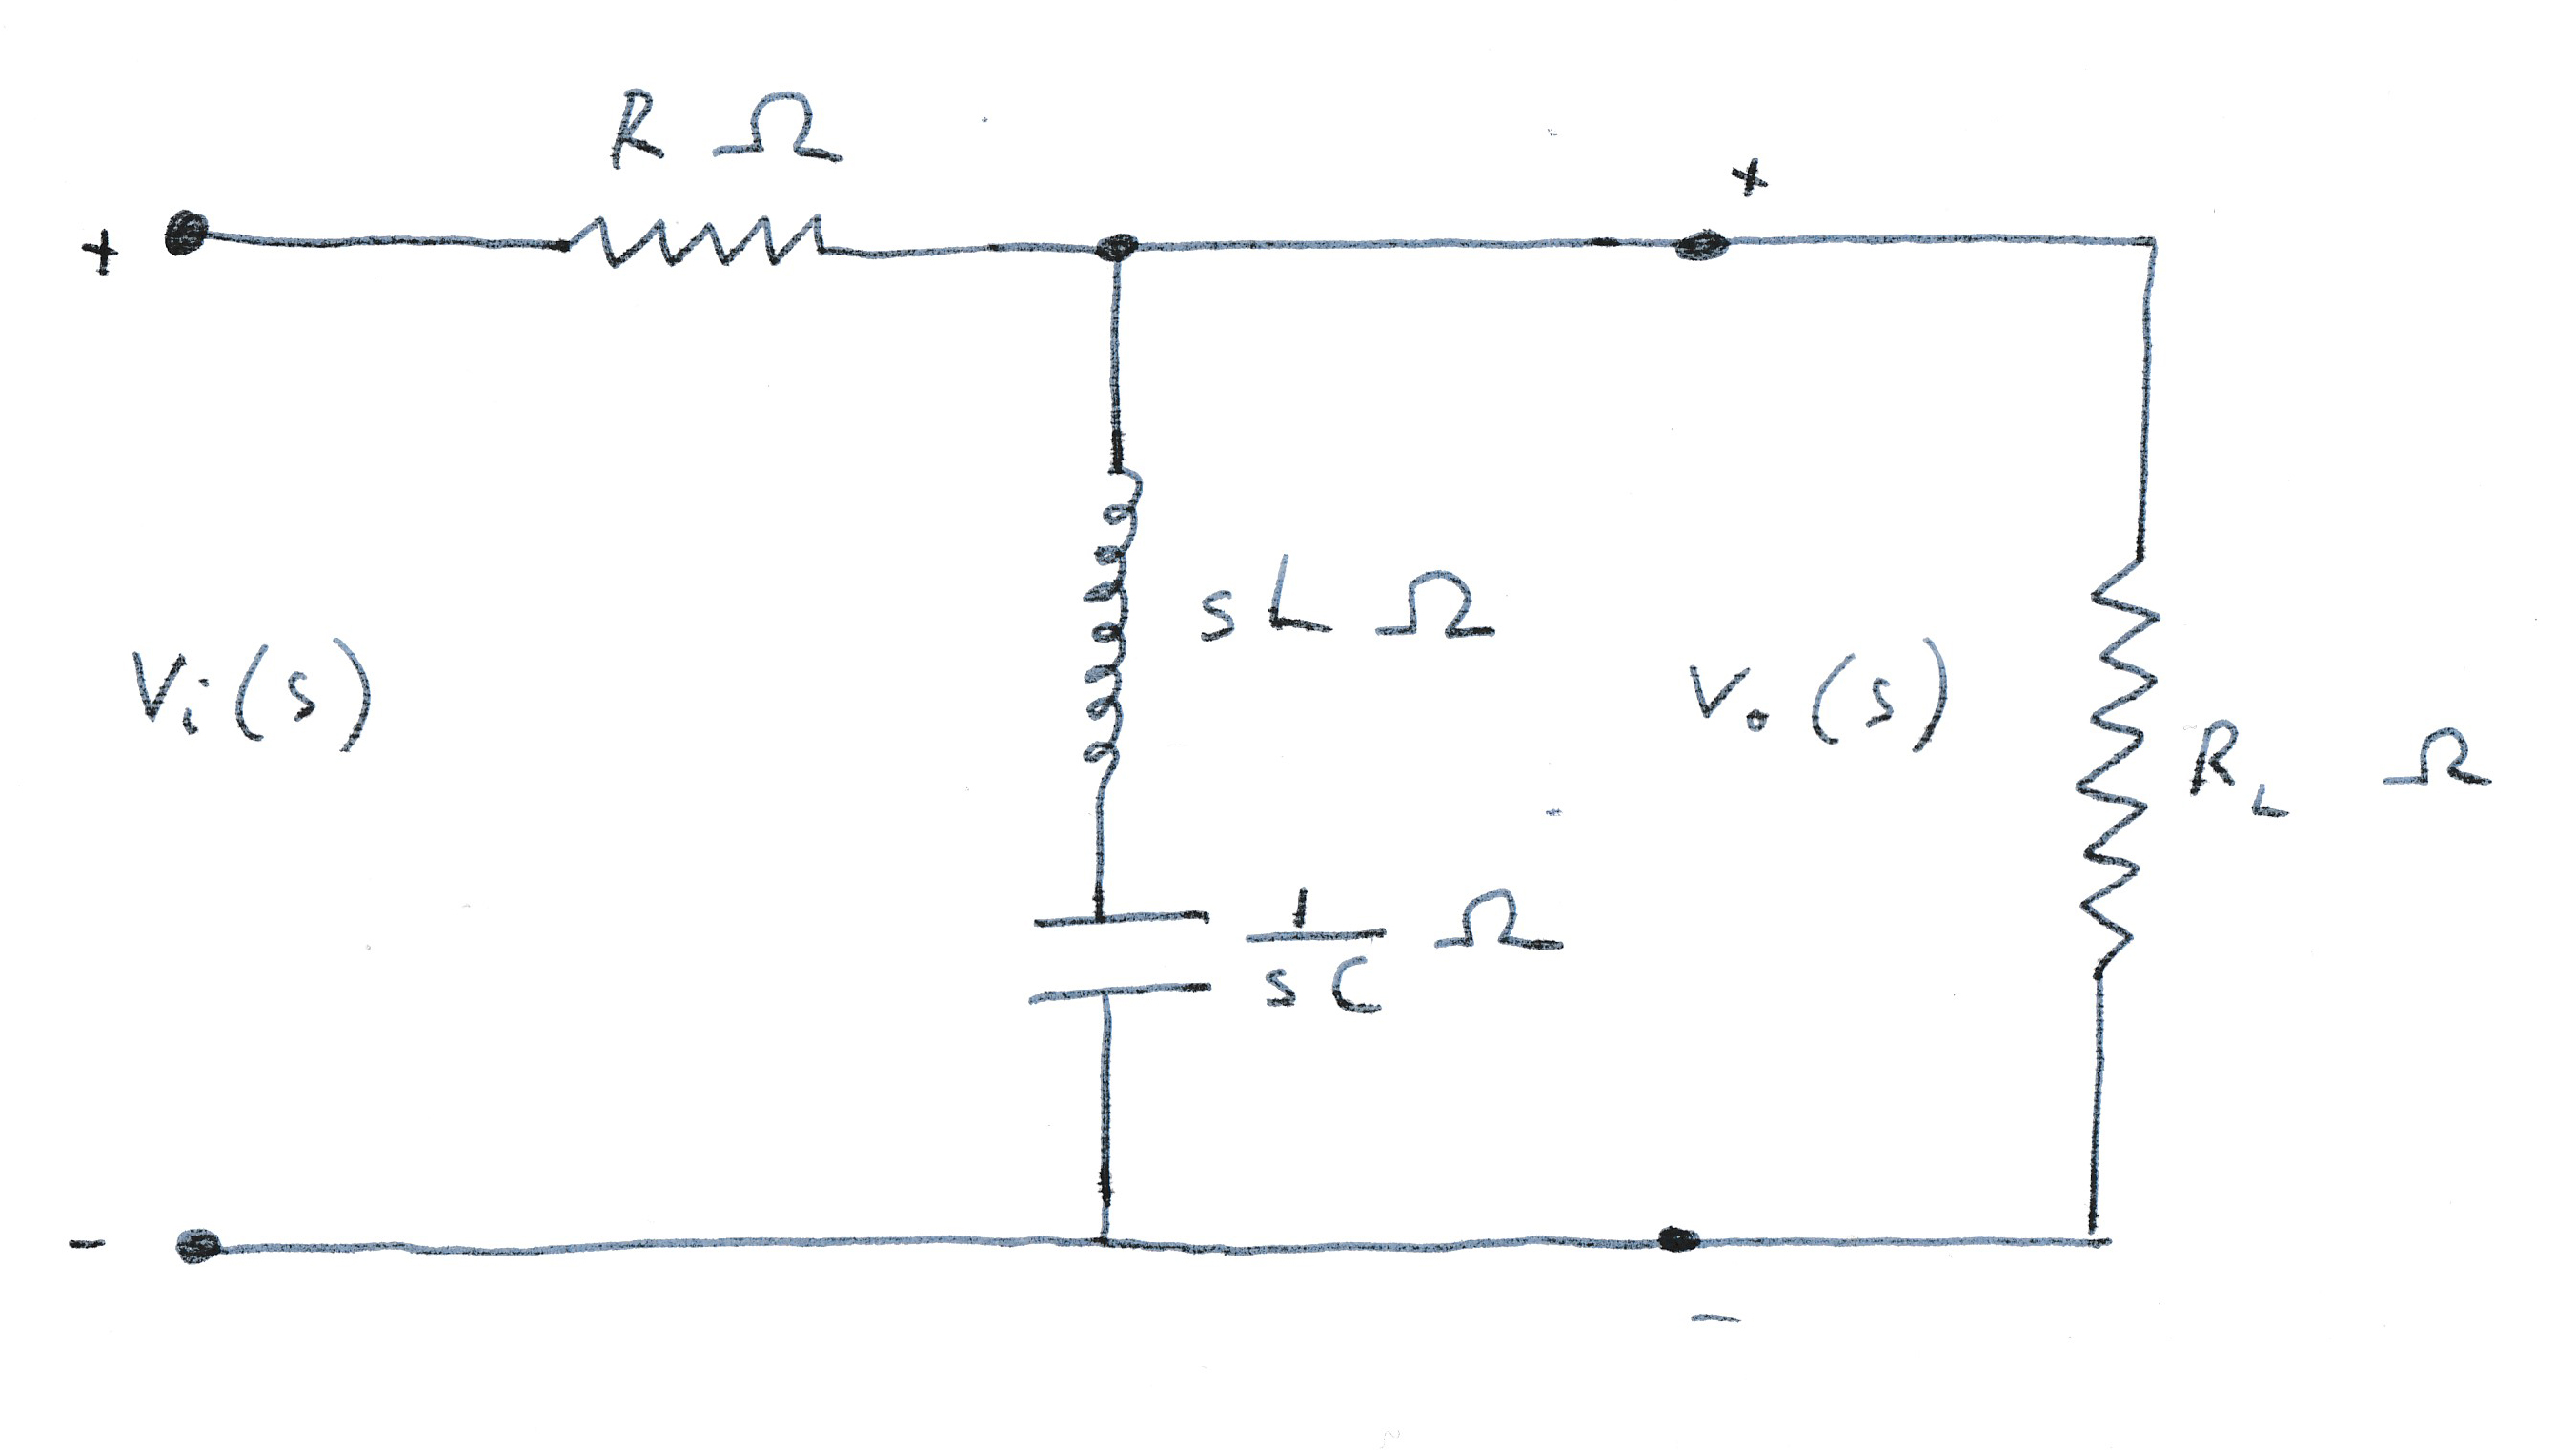
\includegraphics[scale=0.75]{6.JPG}
\end{center}
\end{figure}

Taking $Z_{eq}$ to be the equivalent impedance of the resistor $R_L$, the capacitor and the inductor.
	
\begin{align*}
Z_{eq} &= \left(\frac{1}{R_L} + \frac{1}{sL + \dfrac{1}{sC}}\right)^{-1}\\
&= \left(\frac{1}{R_L} + \frac{1}{\dfrac{s^2LC + 1}{sC}}\right)^{-1}\\
&= \left(\frac{1}{R_L} + \frac{sC}{s^2LC+1} \right)^{-1}\\
&= \left(\frac{s^2LC+1+sR_LC}{R_L(s^2LC+1)} \right)^{-1}\\
&= \frac{R_L(s^2LC+1)}{s^2LC+1+sR_LC}\\
Z_{eq} + R &= \frac{R_L(s^2LC+1)}{s^2LC+1+sR_LC} + R\\
&= \frac{R_L(s^2LC+1) + R(s^2LC+1+sR_LC)}{s^2LC+1+sR_LC}\\
H(s) &= \frac{V_o(s)}{V_i(s)}\\
&= \frac{Z_{eq}}{Z_{eq} + R}\\
&= \frac{R_L(s^2LC+1)}{s^2LC+1+sR_LC} \div \frac{R_L(s^2LC+1) + 
R(s^2LC+1+sR_LC)}{s^2LC+1+sR_LC}\\
&= \frac{R_L(s^2LC+1)}{s^2LC+1+sR_LC} \times 
\frac{s^2LC+1+sR_LC}{R_L(s^2LC+1) + R(s^2LC+1+sR_LC)}\\
&= \frac{R_L(s^2LC+1)}{R_L(s^2LC+1) + R(s^2LC+1+sR_LC)}\\
&=\frac{R_L(s^2LC+1)}{•s^2LC(R+R_L) + sRR_LC + R + R_L}\\
&= \frac{\dfrac{R_L}{R+R_L} (s^2 + \dfrac{1}{LC}) }{s^2 + s \dfrac{RR_L}{L(R + R_L)} + \dfrac{1}{LC}}
\end{align*}